% Options for packages loaded elsewhere
\PassOptionsToPackage{unicode}{hyperref}
\PassOptionsToPackage{hyphens}{url}
%
\documentclass[
  ignorenonframetext,
]{beamer}
\usepackage{pgfpages}
\setbeamertemplate{caption}[numbered]
\setbeamertemplate{caption label separator}{: }
\setbeamercolor{caption name}{fg=normal text.fg}
\beamertemplatenavigationsymbolsempty
% Prevent slide breaks in the middle of a paragraph
\widowpenalties 1 10000
\raggedbottom
\setbeamertemplate{part page}{
  \centering
  \begin{beamercolorbox}[sep=16pt,center]{part title}
    \usebeamerfont{part title}\insertpart\par
  \end{beamercolorbox}
}
\setbeamertemplate{section page}{
  \centering
  \begin{beamercolorbox}[sep=12pt,center]{part title}
    \usebeamerfont{section title}\insertsection\par
  \end{beamercolorbox}
}
\setbeamertemplate{subsection page}{
  \centering
  \begin{beamercolorbox}[sep=8pt,center]{part title}
    \usebeamerfont{subsection title}\insertsubsection\par
  \end{beamercolorbox}
}
\AtBeginPart{
  \frame{\partpage}
}
\AtBeginSection{
  \ifbibliography
  \else
    \frame{\sectionpage}
  \fi
}
\AtBeginSubsection{
  \frame{\subsectionpage}
}
\usepackage{lmodern}
\usepackage{amssymb,amsmath}
\usepackage{ifxetex,ifluatex}
\ifnum 0\ifxetex 1\fi\ifluatex 1\fi=0 % if pdftex
  \usepackage[T1]{fontenc}
  \usepackage[utf8]{inputenc}
  \usepackage{textcomp} % provide euro and other symbols
\else % if luatex or xetex
  \usepackage{unicode-math}
  \defaultfontfeatures{Scale=MatchLowercase}
  \defaultfontfeatures[\rmfamily]{Ligatures=TeX,Scale=1}
\fi
% Use upquote if available, for straight quotes in verbatim environments
\IfFileExists{upquote.sty}{\usepackage{upquote}}{}
\IfFileExists{microtype.sty}{% use microtype if available
  \usepackage[]{microtype}
  \UseMicrotypeSet[protrusion]{basicmath} % disable protrusion for tt fonts
}{}
\makeatletter
\@ifundefined{KOMAClassName}{% if non-KOMA class
  \IfFileExists{parskip.sty}{%
    \usepackage{parskip}
  }{% else
    \setlength{\parindent}{0pt}
    \setlength{\parskip}{6pt plus 2pt minus 1pt}}
}{% if KOMA class
  \KOMAoptions{parskip=half}}
\makeatother
\usepackage{xcolor}
\IfFileExists{xurl.sty}{\usepackage{xurl}}{} % add URL line breaks if available
\IfFileExists{bookmark.sty}{\usepackage{bookmark}}{\usepackage{hyperref}}
\hypersetup{
  pdftitle={305 Lecture 38 - Maximise Expected Utility},
  pdfauthor={Brian Weatherson},
  hidelinks,
  pdfcreator={LaTeX via pandoc}}
\urlstyle{same} % disable monospaced font for URLs
\newif\ifbibliography
\setlength{\emergencystretch}{3em} % prevent overfull lines
\providecommand{\tightlist}{%
  \setlength{\itemsep}{0pt}\setlength{\parskip}{0pt}}
\setcounter{secnumdepth}{-\maxdimen} % remove section numbering
\let\Tiny=\tiny

 \setbeamertemplate{navigation symbols}{} 

% \usetheme{Madrid}
 \usetheme[numbering=none, progressbar=foot]{metropolis}
 \usecolortheme{wolverine}
 \usepackage{color}
 \usepackage{MnSymbol}
% \usepackage{movie15}

\usepackage{amssymb}% http://ctan.org/pkg/amssymb
\usepackage{pifont}% http://ctan.org/pkg/pifont
\newcommand{\cmark}{\ding{51}}%
\newcommand{\xmark}{\ding{55}}%

\DeclareSymbolFont{symbolsC}{U}{txsyc}{m}{n}
\DeclareMathSymbol{\boxright}{\mathrel}{symbolsC}{128}
\DeclareMathAlphabet{\mathpzc}{OT1}{pzc}{m}{it}


% \usepackage{tikz-qtree}
% \usepackage{markdown}
% \usepackage{prooftrees}
% \forestset{not line numbering, close with = x}
% Allow for easy commas inside trees
\renewcommand{\,}{\text{, }}


\usepackage{tabulary}

\usepackage{open-logic-config}

\setlength{\parskip}{1ex plus 0.5ex minus 0.2ex}

\AtBeginSection[]
{
\begin{frame}
	\Huge{\color{darkblue} \insertsection}
\end{frame}
}

\renewenvironment*{quote}	
	{\list{}{\rightmargin   \leftmargin} \item } 	
	{\endlist }

\definecolor{darkgreen}{rgb}{0,0.7,0}
\definecolor{darkblue}{rgb}{0,0,0.8}

\newcommand{\starttab}{\begin{center}
\vspace{6pt}
\begin{tabular}}

\newcommand{\stoptab}{\end{tabular}
\vspace{6pt}
\end{center}
\noindent}


\newcommand{\sif}{\rightarrow}
\newcommand{\siff}{\leftrightarrow}
\newcommand{\EF}{\end{frame}}


\newcommand{\TreeStart}[1]{
%\end{frame}
\begin{frame}
\begin{center}
\begin{tikzpicture}[scale=#1]
\tikzset{every tree node/.style={align=center,anchor=north}}
%\Tree
}

\newcommand{\TreeEnd}{
\end{tikzpicture}
%\end{center}
}

\newcommand{\DisplayArg}[2]{
\begin{enumerate}
{#1}
\end{enumerate}
\vspace{-6pt}
\hrulefill

%\hspace{14pt} #2
%{\addtolength{\leftskip}{14pt} #2}
\begin{quote}
{\normalfont #2}
\end{quote}
\vspace{12pt}
}

\newenvironment{ProofTree}[1][1]{
\begin{center}
\begin{tikzpicture}[scale=#1]
\tikzset{every tree node/.style={align=center,anchor=south}}
}
{
\end{tikzpicture}
\end{center}
}

\newcommand{\TreeFrame}[2]{
\begin{columns}[c]
\column{0.5\textwidth}
\begin{center}
\begin{prooftree}{}
#1
\end{prooftree}
\end{center}
\column{0.45\textwidth}
%\begin{markdown}
#2
%\end{markdown}
\end{columns}
}

\newcommand{\ScaledTreeFrame}[3]{
\begin{columns}[c]
\column{0.5\textwidth}
\begin{center}
\scalebox{#1}{
\begin{prooftree}{}
#2
\end{prooftree}
}
\end{center}
\column{0.45\textwidth}
%\begin{markdown}
#3
%\end{markdown}
\end{columns}
}

\usepackage[bb=boondox]{mathalfa}
\DeclareMathAlphabet{\mathbx}{U}{BOONDOX-ds}{m}{n}
\SetMathAlphabet{\mathbx}{bold}{U}{BOONDOX-ds}{b}{n}
\DeclareMathAlphabet{\mathbbx} {U}{BOONDOX-ds}{b}{n}

\RequirePackage{bussproofs}
\RequirePackage[tableaux]{prooftrees}

\newenvironment{oltableau}{\center\tableau{}} %wff format={anchor = base west}}}
       {\endtableau\endcenter}
       
\newcommand{\formula}[1]{$#1$}

\usepackage{tabulary}
\usepackage{booktabs}

\def\begincols{\begin{columns}}
\def\begincol{\begin{column}}
\def\endcol{\end{column}}
\def\endcols{\end{columns}}

\usepackage[italic]{mathastext}
\usepackage{nicefrac}

\definecolor{mygreen}{RGB}{0, 100, 0}
\definecolor{mypink2}{RGB}{219, 48, 122}
\definecolor{dodgerblue}{RGB}{30,144,255}

\def\True{\textcolor{dodgerblue}{\text{T}}}
\def\False{\textcolor{red}{\text{F}}}

\title{305 Lecture 38 - Maximise Expected Utility}
\author{Brian Weatherson}
\date{July 27, 2020}

\begin{document}
\frame{\titlepage}

\begin{frame}{Plan}
\protect\hypertarget{plan}{}

\begin{itemize}
\tightlist
\item
  In this lecture we'll talk about the relationship between money and
  utility.
\end{itemize}

\end{frame}

\begin{frame}{Associated Reading}
\protect\hypertarget{associated-reading}{}

Section 12.5 of \emph{Odds and Ends}.

\end{frame}

\begin{frame}{Marginal Utility and Decision Making}
\protect\hypertarget{marginal-utility-and-decision-making}{}

\begin{itemize}
\tightlist
\item
  Getting \$2x is not twice as valuable as getting \$x.
\item
  That's because it's like getting \$x, then getting \$x again.
\item
  And after you get the first \$x, you're richer, and getting \$x is (in
  general) less valuable to richer people.
\end{itemize}

\end{frame}

\begin{frame}{Utility and Money}
\protect\hypertarget{utility-and-money}{}

The graph of the relationship between utility and money should have the
following two features.

\begin{enumerate}
\tightlist
\item
  More money means more utility.
\item
  The amount of extra utility you get for each extra dollar should be
  decreasing
\end{enumerate}

Let's look at some familiar mathematical functions that satisfy that
description.

\end{frame}

\begin{frame}{Utility as Square Root}
\protect\hypertarget{utility-as-square-root}{}

\begin{center}


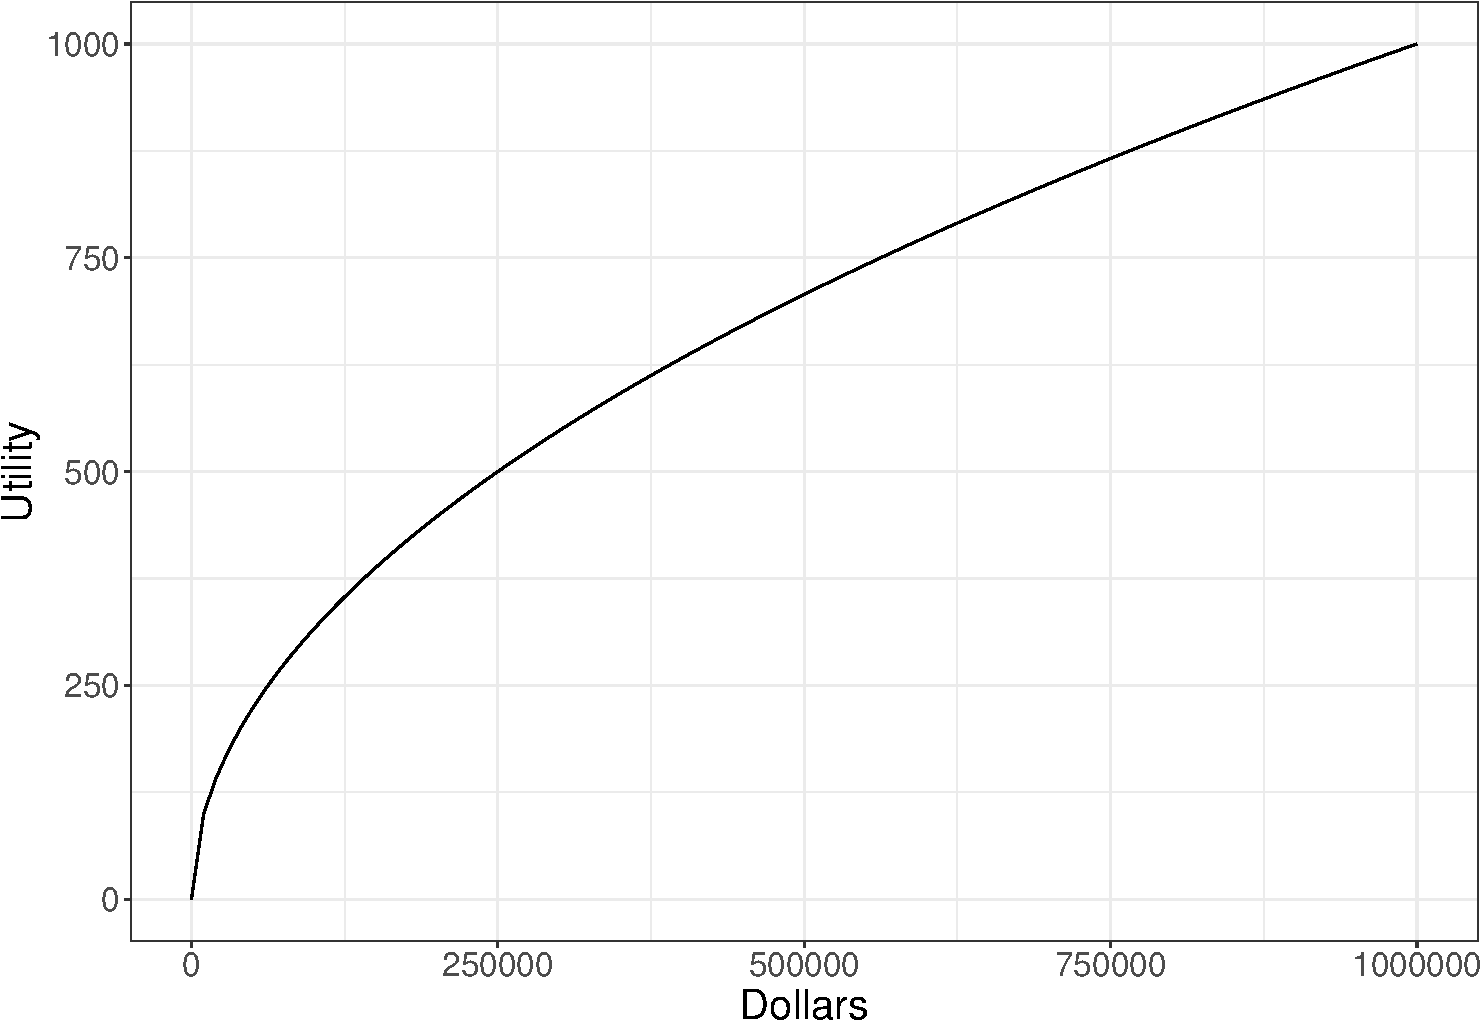
\includegraphics[width=0.9\linewidth]{Lecture_4_m_e_files/figure-beamer/unnamed-chunk-1-1} 

\end{center}

\end{frame}

\begin{frame}{Utility as Square Root}
\protect\hypertarget{utility-as-square-root-1}{}

\begin{itemize}
\tightlist
\item
  This curves down, but not particularly quickly.
\item
  It is a nice toy model of the relationship between utility and money,
  especially because square roots are easy enough to calculate, but it
  isn't that realistic. \pause
\item
  Let's try a different function.
\item
  I'll use a logarithmic function, but I'll ignore values below \$1,000
  because the numbers get weird.
\item
  This is obviously a big thing to ignore!
\end{itemize}

\end{frame}

\begin{frame}{Utility as Log10}
\protect\hypertarget{utility-as-log10}{}

\begin{center}


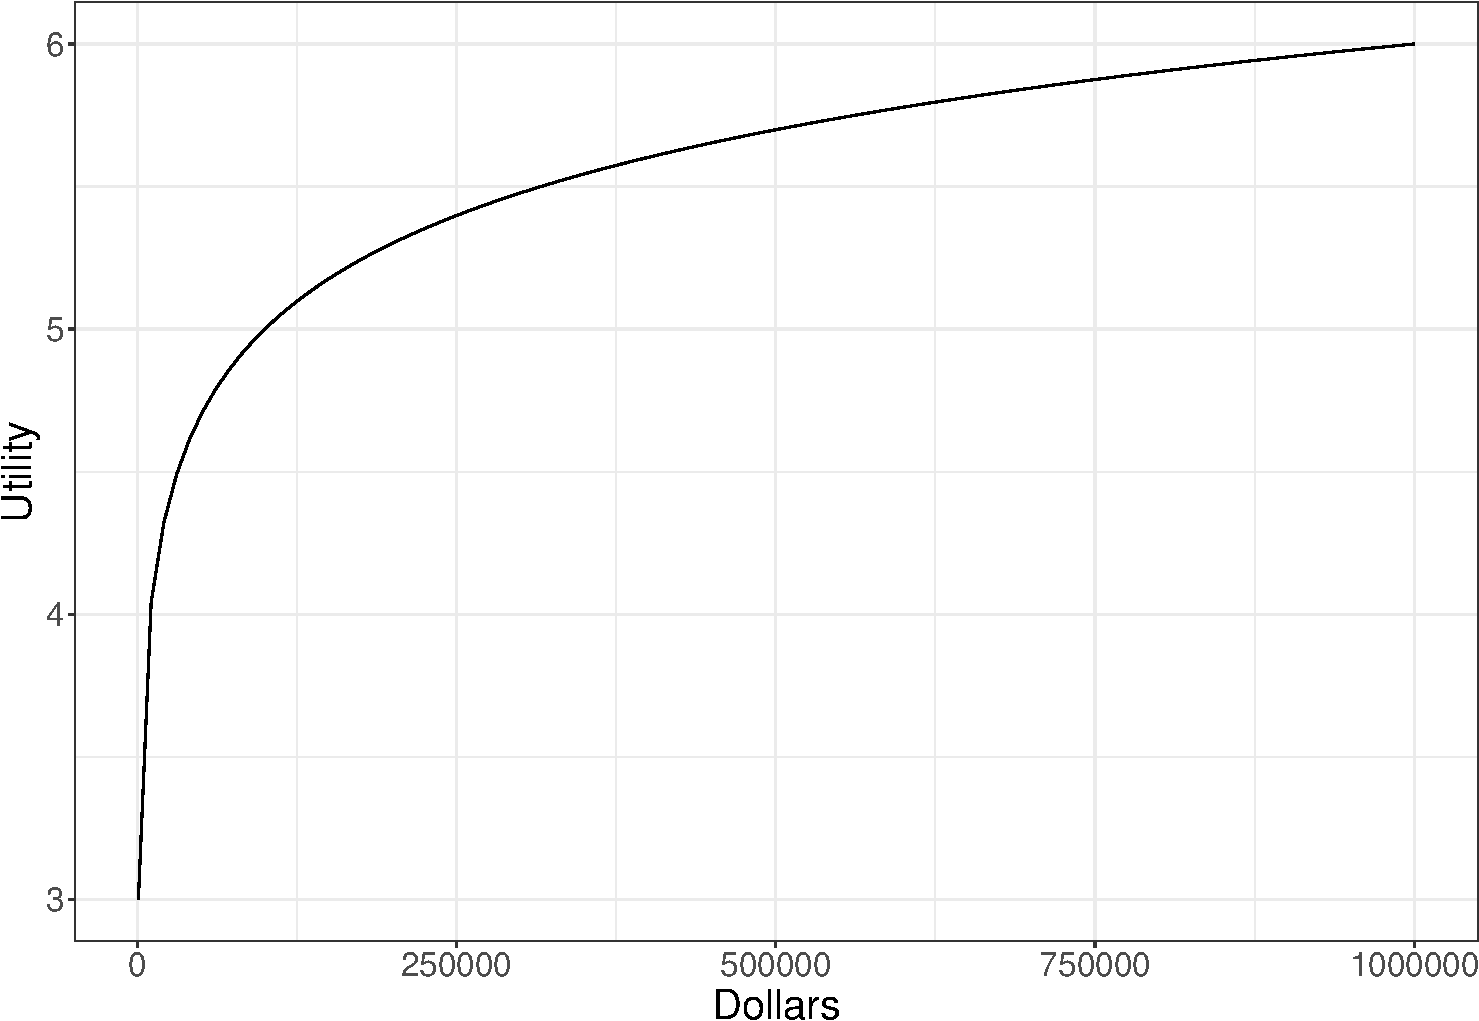
\includegraphics[width=0.9\linewidth]{Lecture_4_m_e_files/figure-beamer/unnamed-chunk-2-1} 

\end{center}

\end{frame}

\begin{frame}{Utility as Log10}
\protect\hypertarget{utility-as-log10-1}{}

\begin{itemize}
\tightlist
\item
  This is a bit more plausible.
\item
  But what about all those dollars below \$1,000?
\item
  Big thing about way to understand these graphs.
\item
  The x-axis measure net total wealth.
\item
  It does not measure size of bank account.
\item
  It includes things like the value of clothes in one's wardrobe, food
  in one's fridge/pantry, dishes/saucepans in one's kitchen etc and, if
  one is particularly wealthy, any means of transportation one has (car,
  bike, etc.).
\item
  Those can fall below \$1,000 - but life is hard below that point.
\end{itemize}

\end{frame}

\begin{frame}{Expected Value of Bets}
\protect\hypertarget{expected-value-of-bets}{}

\begin{itemize}
\tightlist
\item
  Don't think about how much money the bettor stands to gain or lose.
\item
  Instead, think about the possible end-states of the bet.
\end{itemize}

\end{frame}

\begin{frame}{Example (using Log10 Function)}
\protect\hypertarget{example-using-log10-function}{}

Imagine that our person currently has \$100,000 in net wealth. \pause

\begin{itemize}
\tightlist
\item
  They are offered a bet that has a 50\% chance of winning \$900,000,
  and a 50\% chance of losing \$90,000.
\item
  What should they think about the bet?
\end{itemize}

\end{frame}

\begin{frame}{Example (using Log10 Function)}
\protect\hypertarget{example-using-log10-function-1}{}

They should be indifferent between taking and declining the bet.

\begin{itemize}
\tightlist
\item
  Right now, they have utility 5 (i.e., \(log(10^5) = 5\).) \pause
\item
  If they take the bet, they could end up with \$10,000 or \$1,000,000,
  with equal probability.
\item
  That is, they could end up with utility 4 or 6.
\item
  And each of those are equally likely.
\item
  So the expected utility of taking the bet is 5 - just like the status
  quo.
\end{itemize}

\end{frame}

\begin{frame}{Is this Realistic?}
\protect\hypertarget{is-this-realistic}{}

\begin{itemize}
\tightlist
\item
  I'm not sure!
\item
  It seems rather risk averse to me, but the difference in quality of
  life between having \$100,000 and having \$10,000 is pretty
  substantial.
\item
  In one of those you can have a decent car, a nice wardrobe and
  kitchen, and enough spare cash to make rent each month or handle a
  small crisis without problems.
\item
  In the other you can maybe have 1 of those 3.
\end{itemize}

\end{frame}

\begin{frame}{Change the Example}
\protect\hypertarget{change-the-example}{}

Imagine that our person currently has \$100,000 in net wealth.

\begin{itemize}
\tightlist
\item
  They are offered a bet that has a 50\% chance of winning \$800,000,
  and a 50\% chance of losing \$90,000.
\item
  What should they think about the bet? \pause
\item
  It's worse than the previous one, so they shouldn't take it.
\item
  That's even though it's expected dollar return is very very positive.
\end{itemize}

\end{frame}

\begin{frame}{Inverting the Example}
\protect\hypertarget{inverting-the-example}{}

Imagine that our person has \$10,000, plus an asset of very uncertain
value.

\begin{itemize}
\tightlist
\item
  It's got a 50\% chance of being worth nothing, and a 50\% chance of
  being worth \$890,000.
\item
  Someone offers to buy it from them for \$90,000, and they will have no
  other chance to sell it.
\item
  What should they do?
\end{itemize}

\end{frame}

\begin{frame}{Take the Deal}
\protect\hypertarget{take-the-deal}{}

This is just the same as the previous example. They have two choices.

\begin{enumerate}
\tightlist
\item
  A sure \$100,000.
\item
  A 50/50 chance of either \$10,000 or \$900,000.
\end{enumerate}

And they should (given this utility function) take option 1.

\end{frame}

\begin{frame}{Sporting Example}
\protect\hypertarget{sporting-example}{}

\begin{itemize}
\tightlist
\item
  A young pitcher with not many assets (\$10,000 including his old car,
  his sports gear etc) is offered \$90,000 to sign with a pro team.
\item
  He is told, reliably by an agent, that if he plays college ball for a
  year, there's a 50/50 chance that he'll get a great deal next year,
  one worth \$890,000.
\item
  But there's also a 50/50 chance that he'll regress, get injured etc,
  and get nothing.
\item
  What should he do?
\item
  On this model, he should take the deal.
\item
  And of course the team should offer him the deal, even if they think
  there is a 50\% chance that he's of no value to the team.
\end{itemize}

\end{frame}

\begin{frame}{Insurance}
\protect\hypertarget{insurance}{}

Insurance is a funny business.

\begin{itemize}
\tightlist
\item
  Every insurance contract is a bet, with you and the insurance company
  on opposite sides of it.
\item
  The bet can't, as a matter of almost mathematical necessity, have a
  positive expected dollar return for both of you.
\item
  And given it involves some transaction costs, it could have a negative
  expected dollar return for both of you.
\item
  So why does the industry even exist?
\end{itemize}

\end{frame}

\begin{frame}{Declining Marginal Utility}
\protect\hypertarget{declining-marginal-utility}{}

Well let's work through an example.

\begin{itemize}
\tightlist
\item
  Assume our person has assets of \$100,000, including a car worth
  \$30,000.
\item
  They live in a risky area, so there is a 1 in 10 chance the car will
  fall in value to 0 over the next 12 months.
\item
  They are offered an insurance contract with the following terms.
\item
  They pay \$3,200.
\item
  If the risky thing happens and the car value falls to 0, the insurance
  company will reimburse them, so they will get the \$30,000 back.
\end{itemize}

\end{frame}

\begin{frame}{Should They Take the Deal}
\protect\hypertarget{should-they-take-the-deal}{}

Outcome if they take the deal

\begin{itemize}
\tightlist
\item
  A guaranteed \$96,800. \pause
\end{itemize}

Outcome if they don't take the deal.

\begin{itemize}
\tightlist
\item
  A 90\% chance of \$100,000.
\item
  A 10\% chance of \$70,000. \pause
\end{itemize}

The latter outcome has an expected dollar return of \$97,000 - that's
\(0.9 \times 100,000 + 0.1 \times 70,000\).

\end{frame}

\begin{frame}{Should They Take the Deal}
\protect\hypertarget{should-they-take-the-deal-1}{}

\begin{itemize}
\tightlist
\item
  But this doesn't settle the matter. We care about utility not dollars.
\item
  Let's re-run the question using utility.
\end{itemize}

\end{frame}

\begin{frame}{Should They Take the Deal}
\protect\hypertarget{should-they-take-the-deal-2}{}

Outcome if they take the deal

\begin{itemize}
\tightlist
\item
  A guaranteed \$96,800, which has utility roughly 4.986 \pause
\end{itemize}

Outcome if they don't take the deal.

\begin{itemize}
\tightlist
\item
  A 90\% chance of \$100,000, which has utility 5.
\item
  A 10\% chance of \$70,000, which has utility roughly 4.845 \pause
\end{itemize}

The latter outcome has an expected utility return of roughly
\(0.9 \times 5 + 0.1 \times 4.845 \approx 4.984\). Option 1 is better -
not by much, but better.

\end{frame}

\begin{frame}{Company Point of View}
\protect\hypertarget{company-point-of-view}{}

\begin{itemize}
\tightlist
\item
  Assume (for now) that they have a constant marginal utility of money.
\item
  So all that matters is that the policy has a positive dollar value.
\item
  And the expected dollar return of the deal is +\$200, so it's good for
  the company as well.
\end{itemize}

\end{frame}

\begin{frame}{Success!}
\protect\hypertarget{success}{}

\begin{itemize}
\tightlist
\item
  We found a case where both parties are rational in taking the bet,
  even though they are on opposite sides of it.
\item
  And this doesn't require fraud, or misperception of the odds for
  either party.
\end{itemize}

\end{frame}

\begin{frame}{Possibility Constraints}
\protect\hypertarget{possibility-constraints}{}

\begin{itemize}
\tightlist
\item
  This is only possible because the two sides have different utility
  curves, at least locally.
\item
  That's what makes the conflicting interests (in dollar terms) into a
  possible mutual interest.
\item
  Someone with a less steeply sloping utility curve (i.e., with more
  resources) is in a better position to absorb certain risks.
\item
  It is worth paying over the odds to them to absorb that risk.
\end{itemize}

\end{frame}

\begin{frame}{Curves (Almost) Always Slope Down}
\protect\hypertarget{curves-almost-always-slope-down}{}

\begin{itemize}
\tightlist
\item
  But eventually, the insurance company has risks it shudders at as
  well.
\item
  This only happens on enormous scale, but it happens.
\item
  And it's why insurance companies won't (happily) offer insurance
  against correlated risks, like floods or invasion.
\end{itemize}

\end{frame}

\begin{frame}{A Big Caveat}
\protect\hypertarget{a-big-caveat}{}

When you run the numbers on cases like this, three things come out.

\begin{enumerate}
\tightlist
\item
  Sometimes, insurance is good for both parties. \pause
\item
  Unless the loss is a huge portion of the customer's wealth, the
  numbers end up being really close. \pause
\item
  Even in those cases, the numbers aren't that different.
\end{enumerate}

So I end up thinking that people probably over-purchase insurance, even
though this is a model on which insurance purchase can be rational.

\end{frame}

\begin{frame}{For Next Time}
\protect\hypertarget{for-next-time}{}

\begin{itemize}
\tightlist
\item
  We will end today with a famous puzzle about the relationship between
  utility and money.
\end{itemize}

\end{frame}

\end{document}
